%We are generating more data than we could possibly examine.
%	* growth is huge
%	* cite fig
%	* overwhelming ability to analyze/understand

The growth in data-based science has exploded in recent years.  As
Figure~\ref{fig:growth} shows, the size of the available data to
analyze increases exponentially.  While the increased fidelity
enables new levels of understanding, this is only possible if we can
interrogate and analyze the increased scale of data.

\begin{figure}
	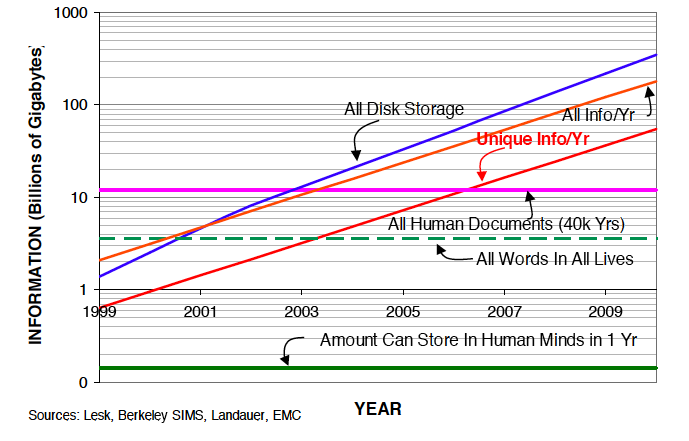
\includegraphics[width=\linewidth]{images/growth}

  \caption{The growth of data in recent years.  Hardware capabilities
  have not kept pace with the exponential pace of data growth.}

	\label{fig:growth}
\end{figure}

Humans are effective pattern recognizers, but error-prone with
repetitive tasks and inherently visual thinkers.  Among even small sets
of data, it is much easier for us to apprehend a change in color than
it is a digit in the third decimal place of a repeated sequences of
numbers.  Mapping raw numbers to color or another visual representation
is thus an effective way to take advantage of the pattern recognition
capabilities of the human visual system.  The growth of data only
increases the need for data visualization, else we will be left with
massive piles of numbers with no insight into the mechanisms or
processes that sourced them.

There are a variety of data types we might apply our efforts to.  In
this thesis, we concentrate on \textit{regular gridded data}, as might
be output by medical (CT, MRI) scanners or used in simulation software.
These kinds of strutured grids account for a disproportionately large
subset of data types used in the scientific and medical domains.  It is
one of the `important' data types highlighted by a report discussing
the future scalability of computing in
science~\cite{Berkeley:2006:View}.  Furthermore, operations on such
data are easily mappable to promising data-parallel hardware, unlike
many other data types, suggesting its continued future use at scale.

%The best-represented subset of scientific data is regularly gridded
%data.
%	* limit ourselves to scientific data
%	* scientific data has spatial and potentially temporal elements
%	* regularly gridded data is disproportionately represented
%	* one of the Berkeley dwarves (5. structured grids)
%	** also fits 1. dense linear algebra

%Berkeley introduces 13 dwarves.
%	 1. dense linear algebra: yes
%	 2. sparse linear alg: no
%	 3. spectral methods: no
%	 4. n-body methods: no
%	 5. structured grids: yes
%	 6. unstructured grids: no
%	 7. monte carlo: no
%	 8. computational logic: no
%	 9. graph traversal: no
%	10. dynamic programming: no
%	11. backtrace, branch+bound: no
%	12. graphical models: no
%	13. finite state machines: no

There are a number of visualization techniques that are widely
appreciated for such volumetric data.  As the techniques have been
known for years, much of the effort has been focused in mapping the
algorithms to novel architectures, identifying special cases of
interest, and reducing constants in the order of the algorithm's
execution.

%Extreme data sizes as well as established algorithms (in SciVis)
%mean there is increasing focus on constants in algorithmic scaling
%equations.
%	* theres exists a small set of `established' vis algorithms
%	* already well-utilized for understanding structured data
%	* known performance/scaling properties
%	* recent/future research focused on reducing constants

% * vis is important
%
% * performance is critical
%
% * prevalence of regular grids

\section{Volume visualization}

%* volume rendering
%	* definition
%	* why is it used
%	* imagevis3d (not tuvok!)

Direct volume rendering produces visualizations that accurately model
tenuous mediums such as fires, smoke, and clouds.  However, it is
seldom applied for its ability to produce photorealistic imagery.  The
scientific and medical domains use volume rendering to see
\emph{inside} a data set and highlight its internal structure.
This can be extremely useful both in interrogating data as well as
communicating known features.

%Volume rendering allows us to see inside data sets.
%	* physically defined for tenuous mediums: fire, smoke, clouds
%	* usually applied elsewhere: CT, MRI, simulation data
%	* can filter out unwanted features
%	* can highlight features of interest

%Volume visualization is a useful technique for understanding the
%structure of 3D data.

The precision instrument used to control volume rendering is called the
\emph{transfer function}.  A transfer function maps the value at every
datum to colors \emph{and} opacities.  The control of opacity gives
users an effective mechanism for filtering out data irrelevant to the
point of interest.  Color control enables the user to specify the
mapping stage of the visualization pipeline.  In contrast to other
volume visualization methods, this gives comparatively more power and
flexibility to the user to communicate a feature exactly as intended.

Unfortunately this increased flexibility comes at the cost of
considerable computational complexity as compared to other volume
visualization techniques.  In the general case, volume rendering is an
$O(n^3)$ algorithm, requiring the consideration of every voxel in a
three-dimensional dataset.  Each of these operations typically consists
of trilinear interpolation coupled with a set of multiply-adds needed
to compute the volume rendering integral.  For data of even modest
size, a na\"ive CPU-based computation will be far from interactive.

%A \emph{transfer function} gives user control over the filtering and
%mapping processes of the visualization pipeline.
%	* tfqn assigns colors and opacities to data values
%	* user control of filtering vis stage
%	* user control of mapping vis stage
%	* thus, precise control over the display

%Volume rendering is computationally complex.
%	* trilinear interpolation
%	* compositing
%	* in general, $O(n^3)$

\section{Systems opportunities}

There are a number of systems-oriented challenges in the ameloriation of
algorithmic constants in volume visualization.

\subsection{Hardware \& programmability}

The end of Moore's law necessitates a reorganization in software
architecture to continue to see performance gains on novel
architectures.  Serial algorithms must be amended to identify
and exploit parallelism, often at multiple scales.  Whereas old
optimization principles emphasized eschewing computation, new
strategies must reduce communication instead.

%	* single processor performance increases have peaked
%	* multiprocessor is the new norm
%	* computation is free, communication costs
%	* limited per-core memory available

Some of the recent research in high-performance computing (HPC) has
been focused on elucidating the appropriate architecture for future HPC
systems.  In part due to the results of this thesis, this architecture
is now known to be based on the `fat node' idea: fewer nodes with
very high levels of shared memory-based concurrency on each node.
Both companies leading the HPC space, NVIDIA and Intel, have invested
heavily in an architecture based on accelerator cards: boards with a
large number of shared memory computational units.  While this is due
in part due to results such as those contained herein, much of this
architecture is dictated by the practical concerns of energy and the
ability to dissipate heat from processing units.

%In part due to the results of this thesis, architecting for
%accelerators as opposed to CPU threads holds greater promise for
%long-term performance scalability.
%	* both leading companies (NVIDIA + intel) have invested in accelerators
%	* accelerator model seems to be here to stay
%	* performance per watt vastly improved

The exact characteristics of accelerators is a current topic of
industry competition, but the general characteristics are large numbers
of low-power cores connected to limited but high-bandwidth memory.
High-powered cores need more power and there are issues dissipating the
heat they generate, so it is unlikely that this basic component of the
architecture will change soon.  Memory faces similar problems, and thus
it seems that the trend of reduced memory per core will continue.

%	* memory is where things get expensive
%	* more powerful cores need more power + can't dissipate heat
%	* but more cores are viable

The challenges these new architectures present gives rise to a number
of programmability concerns.  There are a number of proposals to
ameloriate this problem, but as of yet no solution has arisen as a
clear winner.  Conflating the problem are a number of languages,
libraries, or approaches that are intimately tied with particular
hardware---including CUDA, OpenCL, Threaded Building Blocks (TBB),
OpenMP, OpenAcc, Cilk, and UPC---forcing programmability issues to be
inextricably linked with hardware choices.

%The programmability of future high-performance systems is a competitive
%topic that is presently conflated with that of the hardware.
%	* many library choices
%	** CUDA, OpenCL, Intel TBB, OpenMP, OpenAcc, Cilk, UPC
%	** DAX, EAVL, Piston
%	* hardware choices
%	** CPU threads (dead), GPUs, Xeon Phi

%	* GPUs
%	* versus CPU threads
%	* versus Phi?
%	* future architecture of supercomputers defined by current research
%	* programmability
%	* CUDA, OpenCL, OpenMP, OpenAcc

\subsection{I/O}

The storage hierarchy is the single most limiting factor in
high-performance visualization.  Long term storage is slower than other
subsystems by many orders of magnitude: far wider than the gap between
processor and memory speeds, for example.  Furthermore, there is little
hope that this gap will shrink in the coming years.  This poses a
pernicious problem for visualization, whose primary interaction with
the storage hierarchy is via necessarily synchronous read operations.
Worse, this type of workload is unique to visualization: other
high-performance computing consumers are unlikely to be allies when
negotiating architectural tradeoffs for HPC resources.

%The storage hierarchy is the single most limiting architectural
%component.
%	* slowest component by far
%	* gap between disk and memory is the widest HW gulf
%	* huge problem for vis: synchronous!
%	** vis is unique: no help from general HPC community

While parallel storage continues to make significant progress, the
problems elucidated in recent years are cause for concern.  Parallel
filesystems must intelligently partition and provide access to a
distributed set of disks, but the decomposition of the parallel job
is frequently opaque and only a traditional serial API is presented.
This presents difficulties in avoiding issues such as false sharing or
central and thus contentious repositories for metadata.  At the core of
the issue is the rapidly increasing cost of data movement.

%Parallel storage scalability is not a simple as adding more disks.
%	* data movement is too expensive
%	** must access data intelligently
%	** false sharing
%	* metadata access (storage) is a limiting component
%	* tremendous contention at cluster scales

%* parallel io
%	* filesystems
%	* lustre
%	* MDSs, ODSs or whatever they're called
%	* DDoS metadata
%	* false sharing

There are no imminent advances on the horizon for the storage hierarchy
problems plaguing modern high-performance visualization and analysis
software.  While solid state drives ameloriate some of these concerns,
from a scalability perspective they have only a minor impact.  Given
the realities of current and future architectural limitations, we
must consider alternate approaches to the visualization and analysis
problems.

%There are no imminent advances on the horizon for the IO problems
%plaguing modern visualization and analysis software.
%	* SSDs help, but not nearly enough
%	* only going to get more disks

\subsection{\textit{In situ} visualization}

\textit{In situ} visualization addresses the `too big to read' problem
in large-scale visualization and analysis.  The growing size of outputs
crosses an inflection point relevant to the speed of storage hierarchy.
The simple act of loading data significantly changes the visualization
and analysis workflow.  Past this point, the impracticality of loading
data precludes exploratory visualization and analysis. \textit{In
situ} visualization solves this by foregoing such use cases entirely:
instead, all visualization and analysis is `baked into' the simulation
run itself, running concurrently with the parallel simulation.  The
advantage of this approach is that it obviates the most expensive step
in the majority of visualization pipelines: reading data from disk.

%In situ visualization addresses the `too big to read' problem in
%visualization.
%	* beyond a certain size, it no longer makes sense to read data
% ** waiting to read large data progression: sip your coffee, get a
%    coffee, make a pot, drink a cup, teach a class, sleep, forget it.
%	* in situ solves this by obviating the `read' step

To achieve this coupling of visualization and simulation requires the
combination of software from multiple communities, notably simulation
and visualization \& analysis.  This creates sizable technical and
social challenges.  First and foremost, these are often distinct
groups, with varying research motivations, methods for valuating
engineering contributions, and software processes.  Data models
are often radically different and must be shared across multiple
programming languages.  Finally, large-scale visualization software is
typically large, and both systems tend to have unique but overlapping
dependency stacks.

%In situ visualization exposes difficulties in coupling visualization
%and simulation codes.
%	* typically written by different groups,
%	* in different languages,
%	* with different data models.
%	* visualization software is LARGE and complex

Prior effort into \textit{in situ} visualization is often focused on
scalability and performance.  At the largest scale---the most promising
candidates for benefitting from \textit{in situ} techniques---there is
great concern that visualization will severely impact the execution
time of highly parallel simulation software.  The scalability of these
results is promising, but often comes at large increases in software
complexity and thereby `technical debt'.

%Considerable effort has been focused on scalability and performance.
%	* often serves to make these more complex
%	* cite considerable work in this area

This dissertation is perhaps the first to address the concerns
associated with coupling increasingly complex visualization software
with the simulations it uses as input.  The starting thesis is that
embedding visualization into simulation code should not require a
visualization expert.  It should be possible for the simulation
author or even user to independently perform this task.  Furthermore,
we should measure coupling efforts in hours, not weeks or months.
Starting from
these premises requires a radically different approach to \textit{in
situ} visualization than traditional solutions permit.

%The complexity of modern \textit{in situ} solutions is crippling.
%	* forgotten use case simple code that just wants to do vis
%	* spend more time doing in situ than writing the simulation code
%	* we seem to have forgetten that visualization is a tool to others

%* in situ visualization
%	* solves
%		* data too large to be read
%		* end-to-end 'time-to-insight' performance
%	* problems
%		* how metadata is transferred
%		* vis cannot slow down sim (much)
%		* data access from sim -> vis
%		* difficulty in coupling sim+vis
%		* how often do we update vis
%		* \emph{when} do we update vis

\section{Contribution}

The efforts involved in this dissertation redefined the data sizes
and methods in use to visualize and understand regularly-gridded
three-dimensional data.

\begin{figure}
	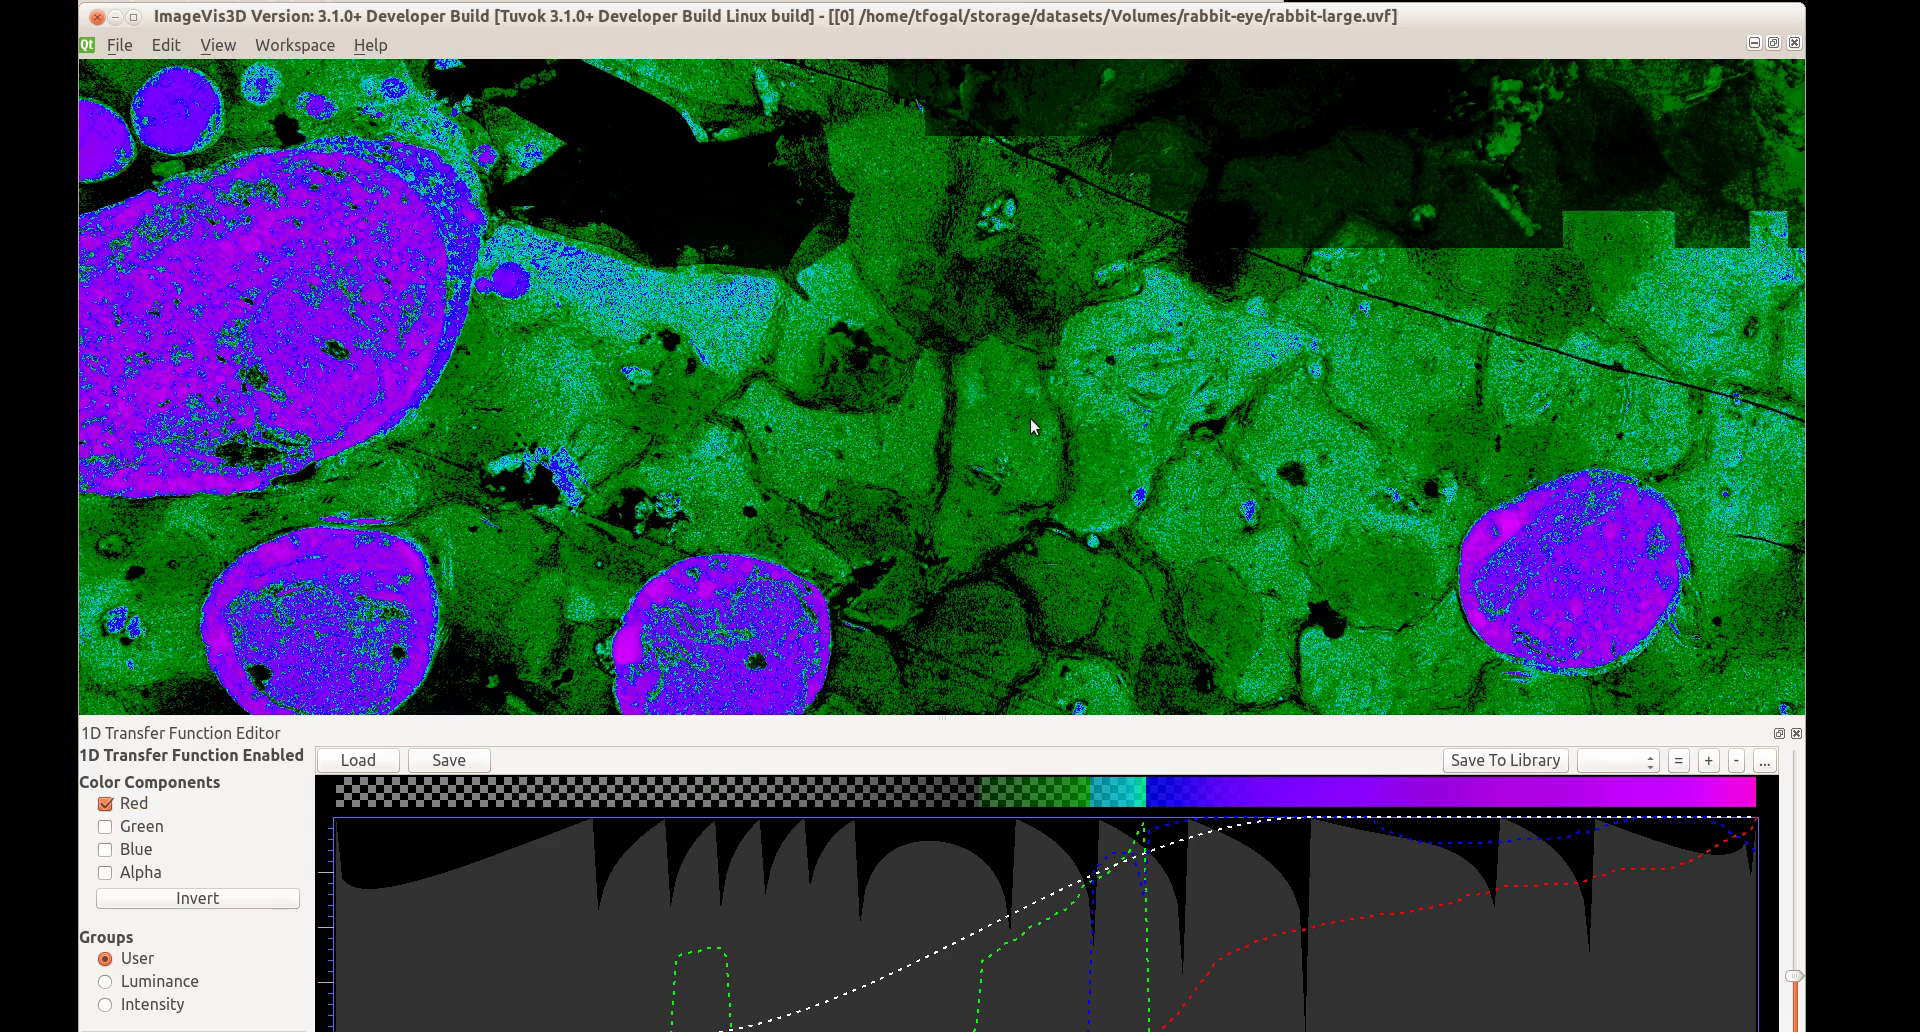
\includegraphics[width=\linewidth]{images/rabbit5tb}

  \caption{ImageVis3D interacting with a 5 terabyte data set of a
  rabbit eye.  The research in this thesis convinced the community
  that what was previously considered `large data' could in fact be
  processed by workstations using commodity hardware.}

	\label{fig:rabbit5tb}
\end{figure}

Prior to the ImageVis3D desktop volume rendering tool developed in
relation to the research appearing here, `large data' visualization was
limited to `big iron' multi-million dollar supercomputing facilities.
Chapters~\ref{chp:tuvok}~and~\ref{chp:rayguided} demonstrate that it
is possible to use workstation computing resources to visualize the
multi-terabyte datasets normally processed on supercomputers, as shown in
Figure~\ref{fig:rabbit5tb}.  Despite
using vastly less hardware, the performance and user experience is even
better than on the large-scale infrastructure.
Chapter~\ref{chp:multiscale} demonstrates that these techniques can
still be applied at scale and uses them to produce the largest-ever
volume renderings, and Chapter~\ref{chp:io} takes that concept further
by investigating the parallel IO concerns at scale.

Volume visualization is simply a means to an end: that of understanding
the structures and processes present in a volume data set.  In recent
years, many have turned to \textit{in situ} visualization to tame the
growing performance concerns of large-scale visualization.  However,
engineering groups have long coupled \textit{ad hoc} visualization and
analysis routines into their simulations to understand their simulation
\emph{while} it runs.  The work developed here in
Chapters~\ref{chp:freeprocessing}~and~\ref{chp:conclusions} is the
first to consider
\textit{in situ} visualization from the engineers' point of view: quick
and easy visualization of their data.

Much of this work has been vetted in field-leading conferences and
journals.
\begin{itemize}

  \item Chapter~\ref{chp:tuvok} is based on, ``Tuvok, an
  Architecture for Large Scale Volume Rendering'' that appeared in VMV
  2010~\cite{Fogal:2010:Tuvok}.

	\item Chapter~\ref{chp:multiscale} is based on, ``Large Data Visualization on
	Distributed Memory Multi-GPU Clusters'' that appeared at HPG
	2010~\cite{Fogal:2010:HPG}.

	\item Chapter~\ref{chp:rayguided} is based on, ``An analysis of scalable
	GPU-based ray-guided volume rendering'' that appeared at LDAV
	2013~\cite{Fogal:2013:Analysis}.

  \item Chapter~\ref{chp:io} is based on, ``Efficient I/O
  for Parallel Visualization'' that was presented at EGPGV
  2011~\cite{Fogal:2011:PracticalIO}.

	\item Chapter~\ref{chp:freeprocessing} is based on,
	``\textit{Free}processing: Transparent \textit{in situ} visualization via
	data interception'' that was presented at EGPGV
	2014~\cite{Fogal:2014:Freeprocessing}.

\end{itemize}

There are also a number of publications by the author that are not considered
`core' components of this thesis~\cite{Fogal:2009:SizeMatters,
Fogal:2010:Bridge, Jevremovic:2011:Education, Jovana:2012:Interactive,
Brownlee:2012:GLuRay, Childs:2012:VisIt, Hermilo:2013:Steering,
Butson:2013:DBS}.  They are mentioned in the text only peripherally.
